\documentclass{article}

%% Language and font encodings
\usepackage[english]{babel}
\usepackage[utf8x]{inputenc}
\usepackage[T1]{fontenc}
\usepackage{amsfonts}
\usepackage[margin=41mm]{geometry}

%% Sets page size and margins
%\usepackage[a4paper,top=3cm,bottom=2cm,left=3cm,right=3cm,marginparwidth=1.75cm]{geometry}

%% Useful packages
\usepackage[colorlinks=true, allcolors=black]{hyperref}
\usepackage{amsmath}
\usepackage{xcolor}
\usepackage{amssymb}
\usepackage{amsthm}
\usepackage{stmaryrd}
\usepackage{graphicx}
\usepackage{enumitem}
\usepackage{tikz, pgfplots}
\usetikzlibrary{positioning}

%Theorem
\newtheorem*{theorem}{Theorem}
\newtheorem*{proposition}{Proposition}
\newtheorem*{lemma}{Lemma}
\newtheorem*{definition}{Definition}
\newtheorem*{corollary}{Corollary}

%Usual Sets
\newcommand{\C}{\mathbb{C}}
\newcommand{\R}{\mathbb{R}}
\newcommand{\Q}{\mathbb{Q}}
\newcommand{\Z}{\mathbb{Z}}
\newcommand{\N}{\mathbb{N}}
\newcommand{\F}{\mathbb{F}}
\newcommand{\E}{\mathbb{E}}
\newcommand{\K}{\mathbb{K}}
\newcommand{\Zn}[1]{\mathbb{Z}/ #1 \mathbb{Z}}

%Special Sets
\newcommand{\Iint}[2]{\llbracket #1 , #2 \rrbracket}

%Math Operators
\let\Re\relax
\let\Im\relax
\DeclareMathOperator{\Im}{\text{Im}}
\DeclareMathOperator{\Re}{\text{Re}}
\DeclareMathOperator{\Null}{\text{null}}
\DeclareMathOperator{\range}{\text{range}}
\DeclareMathOperator{\card}{\text{card}}
\DeclareMathOperator{\Aut}{\text{Aut}}
\DeclareMathOperator{\Hom}{\text{Hom}}
\DeclareMathOperator{\Gal}{\text{Gal}}

%Others
\newcommand{\td}{\textcolor{red}{\textbf{TODO}}}
\newcommand{\isomorphic}{\cong}

%Example environment
\newenvironment{example}{\noindent\textbf{Example:} \vspace{-0.2cm}\begin{itemize}}{\end{itemize}}

%Remark environment
\newenvironment{remark}{\noindent\textbf{Remark:}}{}

%Notation environment
\newenvironment{notation}{\noindent\textit{Notation:}}{}

%Terminology environment
\newenvironment{terminology}{\noindent\textit{Terminology:}}{}

%Set QED symbol to blacksquare
\renewcommand\qedsymbol{$\blacksquare$}


\title{MATH 457 Notes : Galois Theory}
\author{Samy Lahlou}
\date{}

\begin{document}

\maketitle

These notes are based on lectures given by Professor Henri Darmon at McGill University in Winter 2025. The subject of these lectures is Representation Theory and Galois Theory but I chose to only take notes for the Galois Theory part. \\
As a disclaimer, it is more than possible that I made some mistakes. Feel free to correct me or ask me anything about the content of this document at the following address : samy.lahloukamal@mcgill.ca

\tableofcontents

\newpage

\section{Preliminaries}

This section was not part of the lectures but I chose to include it in my notes. The goal is to make an inventory of the non-obvious results used latter that would break the rythm if explained in the middle of the following sections.

\begin{itemize}
    \item Kronecker Construction
    \item Properties of the minimal polynomial over $\F$ of an element in the field extension $\E$.
    \item Given $f,g \in \F[x]$, the difference between the $\gcd$ as polynomials over $\F$ and polynomials over $\E$. Prove that they are equal and hence, the gcd only depends on the ground field. To prove this, $g_{\F}$ divides $g_{\E}$ since it is a polynomial in $\F[x] \subset \E[x]$ which divides both $f$ and $g$. Moreover, $g_{\E}$ divides $g_{\F}$ since $g_{\F}$ can be written as a linear combination of $f$ and $g$. Thus, since they are monic, it follows that $g_{\E} = g_{\F}$.
    \item The cardinality of a field is always a power of a prime.
\end{itemize}

\subsection{Fields}

\td

\begin{theorem}
    Let $\F$ be a finite field, then $\F^{\times}$ is a cyclic group.
\end{theorem}

\begin{proof}
    Since $\F^{\times}$ is a finite abelian group, then we can apply the Fundamental Theorem of Finitely Generated Abelian Groups to obtain that
    $$\F^{\times} \isomorphic \Z^{d_1} \times \dots \times \Z^{d_t}$$
    where $d_i$ divides $d_{i+1}$ for all $i \in \Iint{1}{t-1}$. It follows that $\F^{\times}$ contains an element of order $d_t$ (take $(0,0, ..., 0, 1)$) and every element has an order that divides $d_t$. Thus, $\alpha^n = 1$ for all $\alpha \in \F^{\times}$. Consider the polynomial $p(x) = x^{d_t} - 1 \in \F[x]$, notice that it has at most $\deg p = d_t$ roots and that it all the elements of $\F^{\times}$ are roots so $\# \F^{\times} \leq d_t$. Moreover, since $\F^{\times}$ contains an element of order $d_t$, then it has a subgroup of cardinality $d_t$ which shows that $d_t \leq \# \F^{\times}$. Thus, combining the two previous inequalities, $\F^{\times}$ is a group of cardinality $d_t$ which contains an element of order $d_t$, it follows that $\F^{\times}$ is cyclic.
\end{proof}


\subsection{Irreducible Polynomials}

\td 

\begin{proposition}
    $g(x)$ irreducible if and only if $x^ng(1/x)$ irreducible.
\end{proposition}

\subsection{Formal Derivative and Multiple Roots}

\begin{definition}[Formal Derivative]
    Given a field $\F$ and a polyomial $f(x) = \sum_{i=0}^{n}a_ix^i \in \F[x]$, we define the polynomial $f'(x) = \sum_{i=0}^{n-1}(i+1)a_{i+1}x^i \in \F[x]$ and call it the formal derivative of $f$.
\end{definition}

\begin{proposition}
    Given two polynomials $f,g \in \F[x]$, their respective formal derivatives satisfy the following properties:
    \begin{enumerate}
        \item $(f + g) = f' + g'$.
        \item $(fg)' = f'g + fg'$.
        \item $(f^n)' = nf' f^{n-1}$.
    \end{enumerate}
\end{proposition}

\begin{proof}
    \begin{enumerate}
        \item \td 
        \item \td 
        \item \td
    \end{enumerate}
\end{proof}

\begin{theorem}
    Given a field $\F$, a polynomial $f \in \F[x]$ and a root $\alpha \in \F$ of $f$, then $(x - \alpha)^2$ divides $f$ if and only if $f'(\alpha) = 0$.
\end{theorem}

\begin{proof}
    \td 
\end{proof}

\section{Fields Extensions}

\subsection{Definitions and Examples}

\begin{definition}[Field Extension]
    If and $\E$ and $\F$ are fields, we say that $E$ is an extension of $F$ if $F$ is a subfield of $E$.
\end{definition}

\begin{remark}
    If $\E$ is an extension of $\F$, then $\E$ is also a vector space over $\F$.
\end{remark}

\begin{definition}
    Given fields $\E$ and $\F$ and $\alpha \in \E$ where $\E$ is an extension of $\F$, we denote by $\F[\alpha]$ the ring generated by $\F$ and $\alpha$, i.e., $\F[\alpha]$ is the intersection of all the rings containing both $\F$ and $\alpha$. Similarly, we denote by $\F(\alpha)$ the field generated by $\F$ and $\alpha$.\\
    Hence, there is a natural inclusion from $\F[\alpha]$ to $\F(\alpha)$.
\end{definition}

\begin{definition}
    The degree of $\E$ over $\F$ is the dimension of $\E$ as a $\F$ vector space. It is written as $[\E:\F]$. If the degree is finite, we say that $\E/\F$ is finite. 
\end{definition}

\begin{example}
    \item $[\C : \R] = 2$ since $\R \subset \C$ and $\C$ is a 2-dimensional $\R$-vector space.
    \item $[\C : \Q] = \infty$ since $\Q \subset \C$ and $\C$ is an $\infty$-dimensional $\Q$-vector space. Using the Axiom of Choice, we can construct a basis for this vector space, it is called the Hamel basis.
    \item Let $\F$ be a field and $\E = \F[x]/(p)$ where $p$ is an irreducible polynomial of degree $n$, then 
    $$\E = \{a_0 + a_1x + ... + a_{n-1}x^{n-1}\}$$
    so $[\E : \F] = n$ since $\E$ contains $\F$ (the constant polynomials) and has basis $\{1, x, ..., x^{n-1}\}$.
    \item Let $\F$ be a field and $\E = \F(x)$ be the fraction field of $\F[x]$, then $[\E : \F] = \infty$.
    \item Given an irreducible polynomial $p$ over $\Q$ and a root $\alpha$ of $p$, then 
    $$\Q[\alpha] = \Q(\alpha) = \Q[x] /(p)$$
    is an extension of $\Q$ of degree $\deg p$. The isomorphism $\Q(\alpha) \isomorphic \Q[x] /(p)$ comes from the valuation map $ev_\alpha : \Q[x] /(p) \to \Q(\alpha)$.
\end{example}

\begin{theorem}[Multiplicativity of the degree]
    Given three fields $\K \subset \F \subset \E$, we have
    $$[\E : \K] = [\E : \F] [\F : \K].$$
\end{theorem}

\begin{proof}
    If one of the degree is infinite, the proof is trivial, hence, assume that the degrees are finite. Call $[\E : \F] = n$ and $[\F : \K] = m$. Let $\alpha_1, ..., \alpha_n \in \F$ be a basis for $\E$ as a $\F$-vector space and $\beta_1, ..., \beta_m \in \K$ be a basis for $\F$ as a $\K$-vector space. Notice that for all $a \in \E$, there exist elements $\lambda_1, ..., \lambda_n \in \F$ such that
    $$a = \lambda_1 \alpha_1  + ... + \lambda_n \alpha_n$$
    is the unique representation of $a$ as a linear combination of the basis $\alpha_1, ..., \alpha_n$. But for each $\lambda_i$, we know that there exist elements $\lambda_{i1}, ..., \lambda_{im} \in \K$ such that 
    $$\lambda_i = \lambda_{i1}\beta_1 + ... + \lambda_{im}\beta_m.$$ Thus,
    $$a = \sum_{i=1}^{n}\sum_{j=1}^{m}\lambda_{ij}\alpha_i \beta_j.$$
    Therefore, $\{\alpha_i \beta_j\}_{i,j}$ is a $\K$ basis for $\E$. Hence, it follows that the dimension of $\E$ as $K$-vector space is $n\cdot m$.
\end{proof}

\subsection{Ruler and Compass Constructions}

\begin{definition}
    A complex number is constructible by ruler and compass if it can be obtained from rational numbers by successive applications of field operations (+, -, $\times$, division) and square roots. Using fields, we can say that a number is constructible if it is contained in a sequence of quadratic extensions of $\Q$.
\end{definition}

The set of constructible elements by ruler and compass is an extension of $\Q$ of infinite degree. The goal is to characterize this extension.

\begin{theorem}
    If $\alpha \in \R$ is a root of an irreducible cubic polynomial over $\Q$, then $\alpha$ is not constructible by ruler and compass.
\end{theorem}

\begin{proof}
    Suppose that $\alpha$ is constructible, then there are finite field extensions 
    $$\Q \subset \F_1 \subset ... \subset \F_n$$
    with $\F_{i+1} = \F_i(\sqrt{a_i})$ for some $a_i \in \F_i$. Hence, for all $i$, we have that $[F_{i+1} : F_i] = 2$ since $\{1, \sqrt{a_i}\}$ is a basis for $F_{i+1}$ as a $\F_i$-vector space. Thus, by multiplicativity of the degree, $[\F_n : \Q] = 2^n$. Moreover, we know that $[\Q(\alpha) : \Q] = 3$ so we get the following diagram: 
    \begin{center}
        \begin{tikzpicture}
            %Nodes
            \node at (0,0) (Fn) {$\F_n$};
            \node at (-1.5,-3) (F1) {$\F_1$};
            \node at (-1.5,-0.5) (Fn1) {$\F_{n-1}$};
            \node at (2,-2.5) (Q3) {$\Q(\alpha)$};
            \node at (0,-4) (Q) {$\Q$};

            %Lines
            \draw (Q) -- (Q3) node[midway, above] {\small 3};
            \draw (Q) -- (F1) node[midway, above] {\small 2};
            \draw (Q3) -- (Fn) node[midway, right] {\small $k$};
            \draw (Fn1) -- (Fn) node[midway, above] {\small 2};
            \draw [dashed] (F1) -- (Fn1) node[midway, left] {\small $2^{n-2}$};
        \end{tikzpicture}
    \end{center}
    By the Multiplicativity of the degree, it follows that $2^n = 3k$ which is clearly a contradiction. Therefore, by contradiction, $\alpha$ is not constructible. 
\end{proof}

\begin{example}
    \item (Duplicating the cube) It is equivalent to determine if $\alpha = \sqrt[3]{2}$ is constructible. Notice that $\alpha$ is a root of $p(x) = x^3 - 2$ which is irreducible in $\Q$ so $\alpha$ cannot be constructible.
    \item (Trisection of angle) To prove that it is impossible to trisect angles, let's show in particular that it is impossible to trisect the angle $\theta = 2\pi / 3$. Equivalently, let's determine if $\alpha = \cos (2 \pi / 9)$ is constructible. Recall the following trigonometric identity:
    $$\cos(\theta) = 4 \cos^3 \left(\frac{\theta}{3}\right) - 3\cos \left(\frac{\theta}{3}\right)$$
    which gives us that $\alpha$ is a root of the polynomial $4x^3 - 3x + \frac{1}{2}$. Equivalently, $\alpha$ is a root of the polynomial $p \in \Q[x]$ where $p(x) = 8x^3 - 6x + 1$. Let's prove that $p$ is irreducible over $\Q$. Notice that it is equivalent to prove that the polynomial $q(x) = x^3 - 6x^2 + 8$ is irreducible. Since $q$ has coefficients in $\Z$, then it suffices to show that $q$ is irreducible over $\Z$. To do so, suppose that there exist integers $a,b,c$ such that $q(x) = (x + a)(x^2 + bx + c)$. Regrouping the terms gives us that $ac = 8$ so $a = \pm 1, \pm 2, \pm 4, \pm 8$. However, notice that if we plug-in any of these numbers into $q$, we never get 0, a contradiction. Therefore, $p$ is irreducible so $\alpha$ is not constructible. 
\end{example}

\section{Automorphism Group}

\begin{definition}[Algebraic Numbers]
    Let $\E / \F$ be a finite extension. An element $\alpha \in \E$ is algebraic over $\F$ if $\alpha$ is the root of a polynomial in $\F[x]$.
\end{definition}

\begin{example}
    \item $\sqrt{2} \in \R$ is algebraic over $\Q$ since it solves the polynomial $x^2 - 1 \in \Q[x]$.
    \item $i \in \C$ is algebraic over $\Q$ since it solves the polynomial $x^2 + 1 \in \Q[x]$.
    \item $\pi$ is not algebraic over $\Q$ but it is algebraic over $\Q(\pi^3)$.
    \item The set of $\alpha \in \R$ which are algebraic over $\Q$ is countable (Cantor).
\end{example}

\begin{lemma}
    If $\E / \F$ is a finite extension, then every $\alpha \in \E$ is algebraic over $\F$.
\end{lemma}

\begin{proof}
    Let $\alpha \in \E$ and $n$ be the degree of $\E / \F$, then the set $\{1, \alpha, \alpha^2, ..., \alpha^n\}$ cannot be linearly independent since it contains $n+1$ elements. Hence, there exist scalars $\beta_0, ..., \beta_n \in \F$ such that $\beta_0 + \beta_1 \alpha + \beta_2 \alpha^2 +  ... + \beta_n \alpha^n = 0$. Thus, if we let $p(x) = \beta_0 + \beta_1 x +  ... + \beta_n x^n \in \F[x]$, then $p(\alpha) = 0$ which proves that $\alpha$ is algebraic over $\F$. 
\end{proof}

\begin{definition}[Automorphism Group]
    The automorphism group of $\E / \F$ is
    $$\Aut(\E / \F) = \{\sigma: \E \to \E : \sigma \text{ preserves the operations and } \sigma|_{\F} = \text{id} \}$$
\end{definition}

\begin{proposition}
    If $[\E : \F]$ is finite then $\Aut(\E / \F)$ acts on $\E$ with finite orbits.
\end{proposition}

\begin{proof}
    Let $\alpha \in \E$, let's show that $\alpha$ has only finitely many translates by the action of $\Aut(\E / \F)$. By the previous Lemma, we know that $\alpha$ is algebraic so there is a polynomial $a_n x^n + ... + a_0 \in \F[x]$ satisfied by $\alpha$.  By plugging-in $x = \alpha$, we have
    $$a_n \alpha^n + ... a_1 \alpha + a_0 = 0.$$
    Let $\sigma \in \Aut(\E / \F)$, then applying $\sigma$ on both sides of the previous equation gives us 
    $$\sigma(a_n \alpha^n + ... a_1 \alpha + a_0) = \sigma(0) = 0.$$
    Using the fact that $\sigma$ preserves addition and multiplication, we get
    $$\sigma(a_n)\sigma(a_n)^n + ... + \sigma(a_1)\sigma(\alpha) + \sigma(a_0) = 0.$$
    Finally, since $\sigma$ fixes the elements of $\F$, then 
    $$a_n\sigma(a_n)^n + ... + a_1\sigma(\alpha) + a_0 = 0.$$
    It follows that $\sigma(\alpha)$ must be a root of the same polynomial. Hence, the orbit of $\alpha$ is a subset of the roots of the polynomial that it satisfies (that we fixed at the beginning of the proof). Since polynomials over fields have finitely many roots, then $\alpha$ has a finite orbit.
\end{proof}

\begin{remark}
    Notice that the same proof can be applied if $\E / \F$ is an extension such that all elements of $\E$ are algebraic over $\F$, i.e., if $\E / \F$ is an algebraic extension.
\end{remark}

\begin{theorem}
    If $[\E : \F] < \infty$, then $\#\Aut(\E / \F) < \infty$.
\end{theorem}

\begin{proof}
    Let $\alpha_1, ..., \alpha_n$ be generators for $\E$ over $\F$, then for all $\sigma \in \Aut(\E / \F)$, if we know the behavior of $\sigma$ on the generators, then we know the behavior of $\sigma$ on $\E$. Since there are finitely many generators and each generator has a finite orbit, then there are finitely many possible $\sigma$.
\end{proof}

\begin{example}
    \item Suppose that $\E$ is generated over $\F$ by a single element $\alpha$. Let $p \in \F[x]$ be the minimal polynomial of $\alpha$. Consider the evaluation map 
    \begin{align*}
        ev_{\alpha} &: \F[x] \to \F[\alpha] \\
        f(x) &\mapsto f(\alpha)
    \end{align*}
    We get that $\ker(ev_{\alpha}) = (p)$. Hence, by the isomorphism theorem, $\F[\alpha]/(p) \isomorphic \F[\alpha]$. Since $\F[\alpha]$ is an integral domain, then $\F[\alpha]/(p)$ is an integral domain which is also a finite vector space. Therefore, it is a field and we get that 
    $$\E = \F(\alpha) = \F[\alpha] \isomorphic \F[x]/(p).$$  
\end{example}

\begin{remark}
    Any homomorphism $\phi : \E \to \E$ is automatically injective. If $[\E : \F] < \infty$, then $\phi$ is also surjective since it can also be seen as an injective linear transformation.
\end{remark}

\begin{theorem}
    If $\E/\F$ is a finite field extension, then $\# \Aut(\E / \F) \leq [\E : \F]$.
\end{theorem}

\begin{proof}
    Let's prove by induction on $n$ that $\# \Hom_{\F}(\K, \E) \leq [\K : \F]$ where $\K = \F(\alpha_1, ..., \alpha_n)$. For the case $n=1$, we have $\K = \F(\alpha)$ for some element $\alpha$. We already observed that each $\varphi \in \Hom_{\F}(\K, \E)$ is completely determined by where it maps $\alpha$. Moreover, we know that $\varphi$ must map $\alpha$ to a root of the minimal polynomial $p \in \F[x]$ of $\alpha$ so there are at most $\deg p$ elements in $\Hom_{\F}(\K, \E)$. In other words, $\#\Hom_{\F}(\K, \E) \leq \deg p$. Finally, we also observed that $\K \isomorphic \F[x] / (p)$ so $[\K : \F] = \deg p$. Therefore, $\# \Hom_{\F}(\K, \E) \leq [\K : \F]$. 
    
    For the Induction Step, suppose that it holds for a natural number $n$ and consider case $n+1$. We have $\K = \F(\alpha_1, ..., \alpha_{n+1})$ and define $\F' = \F(\alpha_1, ..., \alpha_n)$. By the Induction Hypothesis, we know that $\# \Hom_{\F}(\F', \E) \leq [\F' : \F]$. If $\F' = \K$, then we are done by the Induction Hypothesis, otherwise, we have $\K = \F'(\alpha_{n+1})$. If we define $d_1 = [\F' : \F]$ and $d_2 = [\K : \F']$, we can visualize the set up so far by the following diagram:
    \begin{center}
        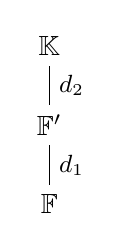
\begin{tikzpicture}
            %Nodes
            \node at (0,-1) (F) {$\F$};
            \node at (0,0) (F') {$\F'$};
            \node at (0,1) (K) {$\K$};

            %Lines
            \draw (F) -- (F') node[midway, right] {\small $d_1$};
            \draw (F') -- (K) node[midway, right] {\small $d_2$};
        \end{tikzpicture}
    \end{center}
    Let $g \in \F'[x]$ be the minimal polynomial of $\alpha_{n+1}$, then $\deg g = [\K : \F'] = d_2$. Write $g$ as
    $$g(x) = \lambda_{d_2}x^{d_2} + \lambda_{d_2 - 1}x^{d_2 - 1} + ... + \lambda_1 x + \lambda_0.$$
    where the $\lambda_i$'s are in $\F'$. We can easily notice that any element of $\Hom_{\F}(\K, \E)$ restricted to $\F'$ is an element of $\Hom_{\F}(\F', \E)$. Hence, to have an estimation on the size of $\Hom_{\F}(\K, \E)$, we can determine in how many ways each element of $\Hom_{\F}(\F', \E)$ can be extended to an element of $\Hom_{\F}(\K, \E)$. Fix a $\varphi \in \Hom_{\F}(\F', \E)$ and let $\varphi_0 \in \Hom_{\F}(\K, \E)$ be an extension of $\varphi$. Notice that for all
    $$K = a_0 + a_1 \alpha_{n+1} + ... + a_{d_2 - 1}\alpha_{n+1}^{d_2 - 1}$$
    in $\K = \F'(\alpha_{n+1})$ where the $a_i$'s are in $\F'$, we can apply $\varphi_0$ to get
    $$\varphi_0(K) = \varphi_0(a_0) + \varphi_0(a_1) \varphi_0(\alpha_{n+1}) + ... + \varphi_0(a_{d_2 - 1}) \varphi_0(\alpha_{n+1})^{d_2 - 1}.$$
    Using the fact that $\varphi_0|_{\F'} = \varphi$, we get
    $$\varphi_0(K) = \varphi(a_0) + \varphi(a_1) \varphi_0(\alpha_{n+1}) + ... + \varphi(a_{d_2 - 1}) \varphi_0(\alpha_{n+1})^{d_2 - 1}.$$
    Since the previous equation expresses $\varphi_0(K)$ in terms of $\varphi_0(\alpha_{n+1})$ for an arbitrary $K \in \K$, then to extend $\varphi$ to $\varphi_0$, it suffices chose where $\alpha_{n+1}$ gets mapped to. From that, recall that $g(\alpha_{n+1}) = 0$ and apply $\varphi_0$ on both sides to obtain
    $$\varphi(\lambda_{d_2})\varphi_0(\alpha_{n+1})^{d_2}  + ... + \varphi(\lambda_1) \varphi_0(\alpha_{n+1}) + \varphi(\lambda_0) = 0.$$
    Thus, if we define $\varphi g \in \E[x]$ as the polynomial $g$ with the coefficients $\lambda_i$ replaced by the coefficients $\varphi(\lambda_i)$, we get that $(\varphi g)(\varphi_0(\alpha_{n+1})) = 0$. It follows that $\varphi_0$ must map $\alpha_{n+1}$ to a root of $\varphi g$ which has degree $d_2$. Since $\varphi_0$ is only determined by its value at $\alpha_{n+1}$, then $\varphi$ can have at most $d_2$ extensions in $\Hom_{\F}(\K, \E)$. Therefore, by the Induction Hypothesis, since there are at most $d_1$ elements in $\Hom_{\F}(\F', \E)$, then by the multiplicativity of the degree:
    $$\#\Hom_{\F}(\K, \E) \leq d_1 d_2 = [\F': \F] [\K : \F'] = [\K : \F].$$
    This concludes our proof by induction. To prove the actual claim, notice that since $\E$ is a finite extension, then it can be written as $\F(\alpha_1, ..., \alpha_n)$ where $\alpha_1, ..., \alpha_{[\E : \F]}$ is the basis of $\E$ as a $\F$-vector space. Therefore, we can plug-in $\K = \E$ to get
    $$\# \Aut(\E / \F) = \# \Hom_{\F}(\E, \E) \leq [\E : \F]$$
    which proves our claim. 
\end{proof}

\section{Galois Extensions} \label{galois_extensions}

\begin{definition}[Galois Extensions]
    An extension $\E / \F$ is a Galois extension if $\# \Aut(\E / \F) = [\E : \F]$. In that case, we write $\Gal(\E / \F)$ to mean $\Aut(\E / \F)$.
\end{definition}

\begin{example}
    \item Take $\E = \C$ and $\F = \R$, then $[\E : \F] = 2$. Moreover, beside the identity from $\C$ to $\C$, we know that the conjugation map is contained in $\Aut(\C / \R)$. Therefore, $\Aut(\C / \R)$ contains two maps so $\Aut(\C / \R)$ is a Galois extension. 
    \item Take $\F = \Q$ and $\E = \Q(\sqrt[3]{2}) \subset \R$, then the automorphisms in $\Aut(\E / \F)$ must map $\sqrt[3]{2}$ to a root of $x^3 - 2$ in $\E$. However, $\sqrt[3]{2}$ is the only element of $\Q(\sqrt[3]{2})$ with this property. Therefore, $\Aut(\E / \F)$ only contains the identity map. It follows that this extension is not Galois.
    \item Let $\zeta$ be a cube root of 1 distinct than 1, then the minimal polynomial of $\zeta$ over $\Q$ can be found by writing
    $$\zeta^3 - 1 = 0 \implies (\zeta - 1)(\zeta^2 + \zeta + 1) = 0 \implies \zeta^2 + \zeta + 1 = 0$$
    and noticing that $x^2 + x + 1$ is irreducible oever $\Q$ (since it is irreducible over $\R$). It follows that the minimal polynomial of $\zeta$ is $p(x) = x^2 + x + 1$. Hence, $\Q(\zeta) \subset \C$ is an extension of $\Q$ of degree $2$. Similarly, if we consider the extension $\Q(\sqrt[3]{2}, \zeta) = \Q(\sqrt[3]{2})(\zeta)$ of $\Q(\sqrt[3]{2})$, then $p$ stays irreducible so this extension also has degree 2. Therefore, by the following diagram and by the multiplicativity of the degree, $\Q(\sqrt[3]{2}, \zeta)$ is an extension of $\Q(\zeta)$ of degree 2:
    \begin{center}
        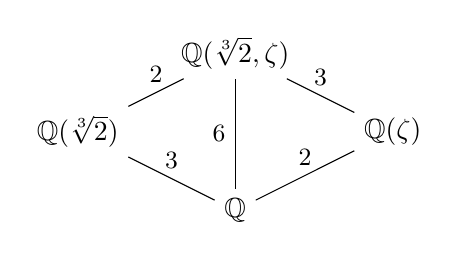
\begin{tikzpicture}
            %Nodes
            \node at (0,-1) (Q) {$\Q$};
            \node at (-2,0) (Qs) {$\Q(\sqrt[3]{2})$};
            \node at (2,0) (Qz) {$\Q(\zeta)$};
            \node at (0,1) (Qsz) {$\Q(\sqrt[3]{2}, \zeta)$};

            %Lines
            \draw (Q) -- (Qs) node[midway, above] {\small $3$};
            \draw (Q) -- (Qz) node[midway, above] {\small $2$};
            \draw (Q) -- (Qsz) node[midway, left] {\small $6$};
            \draw (Qs) -- (Qsz) node[midway, above] {\small $2$};
            \draw (Qz) -- (Qsz) node[midway, above] {\small $3$};
        \end{tikzpicture}
    \end{center}
    Let's count the number of elements in $\Aut(\Q(\sqrt[3]{2}, \zeta) / \Q)$. Let $\phi \in \Aut(\Q(\sqrt[3]{2}, \zeta) / \Q)$, then $\varphi(\zeta)$ must be a root of $x^2 + x + 1$ so $\varphi(\zeta)$ can be mapped to $\zeta$ and $\overline{\zeta}$. Similarly, $\sqrt[3]{2}$ must be mapped to a root of $x^3 - 2$. But since $\zeta^3 = 1$, then $\varphi(\sqrt[3]{2})$ can be $\sqrt[3]{2}$, $\zeta\sqrt[3]{2}$ or $\overline{\zeta} \sqrt[3]{2}$. Since $\varphi$ is only determined by $\varphi(\zeta)$ and $\varphi(\sqrt[3]{2})$, then there are 6 elements in $\Aut(\Q(\sqrt[3]{2}, \zeta) / \Q)$. Therefore, it is a Galois extension. 
    \item Let's determine the structure of $G = \Gal(\Q(\sqrt[3]{2}, \zeta) / \Q)$. Since it has cardinality 6, then it is either $\Zn{6}$ or $S_3$. Let's show that it is $S_6$ by showing that no element has order 6. Let $\varphi \in G$, if $\varphi(\zeta) = \zeta$ or $\varphi(\sqrt[3]{2}) = \sqrt[3]{2}$, then $\varphi$ has at most order 3. Hence, the only possible candidates for an element of order 6 in $G$ are $\varphi_1$ and $\varphi_2$ where $\varphi_1(\zeta) = \varphi_2(\zeta) = \overline{\zeta}$, $\varphi_1(\sqrt[3]{2}) = \zeta \sqrt[3]{2}$ and $\varphi_2(\sqrt[3]{2}) = \overline{\zeta} \sqrt[3]{2}$. Notice that in both cases, $\overline{\zeta}$ is mapped to $\zeta$ because it can only be mapped to a root of $x^2 + x + 1 = (x - \zeta)(x - \overline{\zeta})$ and if it was mapped to $\overline{\zeta}$, then it would break the fact that it is injective. Hence,
    $$\varphi_1^2(\zeta) = \varphi_1(\overline{\zeta}) = \zeta \quad \text{ and }\quad \varphi_1^2(\sqrt[3]{2}) = \varphi_1(\zeta)\varphi_1(\sqrt[3]{2}) = \overline{\zeta}\zeta \sqrt[3]{2} = \sqrt[3]{2}$$
    and 
    $$\varphi_2^2(\zeta) = \varphi_2(\overline{\zeta}) = \zeta \quad \text{ and }\quad \varphi_2^2(\sqrt[3]{2}) = \varphi_2(\overline{\zeta})\varphi_2(\sqrt[3]{2}) = \zeta \overline{\zeta} \sqrt[3]{2} = \sqrt[3]{2}$$
    so $\varphi_1^2 = \varphi_2^2 = id$. Thus, both $\varphi_1$ and $\varphi_2$ have order 2. It follows that $G$ has no element of order 6 so $G$ must be $S_3$. 
\end{example}

Galois Extensions can be seen as field extensions on which we can be read off a lot of structure and properties from the symmetries. The next theorem justifies this way of thinking about Galois extensions. In the next propositions and definitions, fix a field $\F$, a finite Galois extension $\E$ and denote by $G$ the Galois Group of $\E / \F$. \\

\begin{notation}
    $\E^G = \{\alpha \in \E : g(\alpha) = \alpha \text{ for all } g\in G\}$ is the set of fixed points of $G$.
\end{notation}

\begin{lemma}
    $\E^G$ is a subfield of $\E$ which contains $\F$.
\end{lemma}

\begin{proof}
    All the elements of $\F$ are fixed by all the elements of $G$ so $\F \subset \E^G$. Moreover, by definition, we already know that $\E^G \subset \E$. Hence, it remains to show that $\E^G$ is a subfield of $\E$, i.e., that $\E^G$ contains 0, 1, is closed under addition, multiplication and respective inverses. Since $\F \subset \E^G$, then in particular $0,1 \in \E^G$. Since the elements of $G$ are field homomorphisms, then for all $x,y \in \E^G$ and $\varphi \in G$, we have $\varphi(x + y) = \varphi(x) + \varphi(y) = x + y$ and $\varphi(xy) = \varphi(x)\varphi(y) = xy$ so $\E^C$ is closed under addition and multiplication. Similarly, for all $x,y \in \E^G$ with $y \neq 0$ and $\varphi \in G$, we have $\varphi(-x) = -\varphi(x) = -x$ and $\varphi(y^{-1}) = \varphi(y)^{-1} = y^{-1}$ so $\E^G$ is closed under additive and multiplicative inverses. Therefore, $\E^G$ is a subfield of $\E$.
\end{proof}

\begin{theorem}
    $\E^G = \F$.
\end{theorem}

\begin{proof}
    By the previous lemma, we have the following tower of extensions
    \begin{center}
        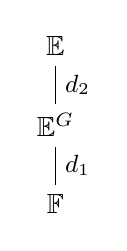
\begin{tikzpicture}
            %Nodes
            \node at (0,-1) (F) {$\F$};
            \node at (0,0) (F') {$\E^G$};
            \node at (0,1) (K) {$\E$};

            %Lines
            \draw (F) -- (F') node[midway, right] {\small $d_1$};
            \draw (F') -- (K) node[midway, right] {\small $d_2$};
        \end{tikzpicture}
    \end{center}
    where $d_1 = [\E^G : \F]$ and $d_2 = [\E : \E^G]$. Let's show that $d_1 = 1$. Consider the set $\Aut(\E / \E^G)$, then it must contain $G$. Moreover, by the last theorem of the previous section, $\# \Aut(\E / \E^G) \leq d_2 = [\E : \E^G] \leq [\E : \F]$. Thus, we obtain:
    $$[\E : \F] = \# G \leq \# \Aut(\E / \E^G) \leq [\E : \F]$$
    which implies that $\# \Aut(\E / \E^G) = [\E : \E^G] = d_1 d_2 \leq d_2$. It follows that $d_1 = 1$. 
\end{proof}

\begin{theorem}
    If $f$ is an irreducible polynomial in $\F[x]$ which has a root in $\E$, then $f$ splits completely into linear factors in $\E[x]$. 
\end{theorem}

\begin{proof}
    Let $r \in \E$ be a root of $f$, then it is easy to see (using the Euclidean Algorithm) that $f$ is the minimal pokynomial of $r$ over $\F$. Consider the orbit $\{r_1, ..., r_n\}$ of $r$ under the action of $G$ on $\E$ and define the polynomial $g(x) = \prod(x - r_i) \in \E[x]$. Notice that if we expand the product, we get that $g(x) = x^n - \sigma_1 x^{n - 1} + ... + (-1)^n \sigma_n$ where the $\sigma_i$'s are the elementary symmetric functions in $r_1, ..., r_n$. It follows that for all $1 \leq i \leq n$, $\sigma_i \in \E^G = \F$ since by symmetry $\sigma_i$ is fixed by all the elements of $G$. Thus, $g \in \F[x]$ with $g(r) = 0$ so it follows by minimality of $f$ that $f$ divides $g$. Therefore, in $\E[x]$, $f$ divides a product of linear factors so $f$ must itself be a product of linear factors. Hence, $f$ splits completely in $\E[x]$. 
\end{proof}

\begin{terminology}
    If a field extension has the property that any irreducible polynomial with the polynomial ring of the ground field with a root in the extension splits completely in the polynomial ring of the extension, we say that the extension is normal. \\
\end{terminology}

Using this terminology, the previous theorem states that any Galois extension is normal.

\section{Splitting Fields}

\subsection{Existence and Uniqueness}

\begin{definition}
    Given a field $\F$ and a polynomial $f \in \F[x]$, a splitting field of $f$ is an extension $\E / \F$ satisfying
    \begin{enumerate}[label=(\alph*)]
        \item $f$ factors into linear factors in $\E[x]$.
        \item $E$ is generated as a field by the roots $r_1, ..., r_n$ of $f$.
    \end{enumerate}
\end{definition}

\begin{theorem}[Existence]
    Given a field $\F$ and a polynomial $f$, there exists an extension $\E / \F$ which is a splitting field of $f$.
\end{theorem}

\begin{proof}
    Let's prove it by induction on the degree of $f$. For the base case, $n=1$, if $f$ has degree 1, then its unique root $r$ must be in $\F$ already so $\E = \F(r) = \F$ is a splitting field of $f$. For the Inductive Step, assume that the statement holds for polynomials of degree $n$ and suppose that $f$ has degree $n+1$. Let $p$ be an irreducible factor of $f$ and construct the field $L = \F[x]/(p) = \F(r_0)$ which contains a root $r_0$ of $p$. It follows that $f(x)$ can be written as $(x - r)g(x)$ in $L[x]$ where $g$ has degree $n$. Hence, by applying the inductive hypothesis, we can construct a splitting field $\E / L$ of $g$. It follows that $g(x)$ can be written as $(x - r_1) \dots (x - r_n)$ in $\E[x]$ so $f(x)$ splits completely into $(x - r_0)(x - r_1) \dots (x - r_n)$ in $\E[x]$. Moreover, since $\E$ is generated by $L$ and the roots of $g$, then
    $$\E = L(r_1, ..., r_n) = \F(r_0)(r_1, ..., r_n) = \F(r_0, r_1, ..., r_n)$$
    which proves that $\E$ is generated by the roots of $f$. Therefore, by induction, we can always construct a splitting field given a field $\F$ and a polynomial $f \in \F[x]$.
\end{proof}

\begin{remark}
    It is very hard to compute the degree of a splitting field since it depends very subtly on the structure of $f$. However, by the multiplicativity of the degree, the degree of the splitting field must be smaller than $(\deg f)!$.
\end{remark}

\begin{theorem}[Uniqueness]
    Given a field $\F$, a polynomial $f \in \F[x]$ and two splitting fields $\E$ and $\E'$ of $f$ over $\F$, then $\E$ and $\E'$ are isomorphic as extensions of $\F$, i.e., there exists a field isomorphism from $\E$ to $\E'$ that fixes $\F$.
\end{theorem}

\begin{proof}
    Let's proceed by induction on $n = \deg f$. For the base case, if $\deg f = 1$, then we simply have $\E = \F = \E'$ so we are done. Assume now that the claim holds for $n$ and suppose that $\deg f = n+1$. Let $p \in \F[x]$ be an irreducible factor of the polynomial $f$, let $r$ be a root of $p$ in $\E$ and let $r'$ be a root of $p$ in $\E'$. We have the following diagram:
    \begin{center}
        \begin{tikzpicture}
            %Nodes
            \node at (0,-1.5) (F) {$\F$};
            \node at (-1.5,0) (Fr) {$\F(r)$};
            \node at (-1.5,1.5) (E) {$\E$};
            \node at (1.5,0) (Fr') {$\F(r')$};
            \node at (1.5,1.5) (E') {$\E'$};

            %Lines
            \draw (F) -- (Fr);
            \draw (F) -- (Fr');
            \draw (Fr) -- (E);
            \draw (Fr') -- (E');
            \draw [dashed, ->] (Fr) -- (Fr') node[midway, above] {\small $\varphi$};
        \end{tikzpicture}
    \end{center}
    Notice that both $\F(r)$ and $\F(r')$ are isomorphic to $\F[x]/(p)$ so in particular, $\F(r) \isomorphic \F(r')$. Let $\varphi : \F(r) \to \F(r')$ be such an isomorphism. Hence, if we let $L = \F(r) = \F(r')$, our diagram becomes
    \begin{center}
        \begin{tikzpicture}
            %Nodes
            \node at (0,-1.5) (F) {$\F$};
            \node at (0,0) (L) {$L$};
            \node at (-1.5,1.5) (E) {$\E$};
            \node at (1.5,1.5) (E') {$\E'$};

            %Lines
            \draw (F) -- (L);
            \draw (L) -- (E);
            \draw (L) -- (E');
        \end{tikzpicture}
    \end{center}
    It follows that $\E$ and $\E'$ can be seen of splitting fields of a polynomial in $L[x]$ of degree $n$ so by the inductive hypothesis, $\E$ and $\E'$ are isomorphic as extensions of $L$. Therefore, $\E$ and $\E'$ are isomorphic as extensions of $\F$. 
\end{proof}

We can now talk about \textit{the} splitting field of a polynomial $f$ over a field $\F$. The next theorem justifies the link between splitting fields and Galois extensions. 

\begin{proposition}
    If $\E / \F$ is Galois, then $\E$ is the splitting field of a polynomial $f \in \F[x]$.
\end{proposition}

\begin{proof}
    Since $[\E : \F] < \infty$, then we can let $\alpha_1, ..., \alpha_n$ be a finite set of generators for $\E / \F$. Since every element of $\E$ is algebraic over $\F$, then we can let $f_1, ..., f_n$ be irreducible polynomials in $\F[x]$ having respective roots $\alpha_1, ..., \alpha_n$ and define $f = f_1 \cdot \dots \cdot f_n$. In $\E[x]$, all the $f_i$'s factor completely and therefore so does $f$. Moreover, the roots of $f$ in $\E$ generate $\E$ so $\E$ is the splitting field of $f$ over $\F$.
\end{proof}

\subsection{Application to Finite Fields}

Recall that if $\F$ is a finite field, then it must have a charachteristic equal to a prime number $p$ which implies that $\F$ contains a copy of $\Zn{p}$. From this, we can see $\F$ as a vector space over $\Zn{p}$ which implies that $\# \F$ must be a power of $p$. However, given any prime power $p^n$ can we construct fields of cardinality $p^n$ ? Are they necessarily isomorphic one to another ?

\begin{theorem}
    Given a prime $p$ and a natural number $n$, there is a unique field of cardinality $p^n$ up to isomorphism.
\end{theorem}

One possible approach would be to find a polynomial $f \in \F_p[x]$ which is irreducible of degree $n$ and construct $\F = \F_p[x] / (f)$ which is the desired field. However, it is not clear that there exists such a polynomial $f$ or there might be several of them. We will not use this approach in the proof. The theory of splitting fields we developed gives us the perfect tools to prove this theorem. 

\begin{proof}
    Let $\F$ be the splitting field of $f(x) = x^{p^n} - x \in \F_p[x]$, let's show that $\F$ has cardinality $p^n$. First, notice that $f$ has distinct roots in $\F$ since its formal derivative is identically $-1$ (so no multiple roots). Since $f$ splits completely in $\F$, then $f$ has $p^n$ roots $\alpha_1, ..., \alpha_{p^n}$. But notice that the roots of $f$ in $\F$ form a field which contains $\F_p$. It follows that $\F = \F_p(\alpha_1, ..., \alpha_{p^n})$ is simply the set of roots of $f$ in $\F$. Therefore, $\F$ has cardinality $p^n$ which proves the existence part of the claim.
    
    Now, let $\F'$ be a field of cardinality $p^n$, then $\F'$ must have characteristic $p$ (because we know that $\# \F' = q^m$ where $q$ is its characteristic which is a prime number, $q^m = p^n \implies \text{char}(\F') = p$). It follows that $\F'$ contains $\F_p$ as a subfield so it is an extension of $\F_p$. Moreover, notice that all the elements of $\F'$ are roots of the polynomial $f(x) = x^{p^n} - x \in \F_p[x]$ so $f$ splits completely in $\F'$ (since $\# \F' = \deg f$). And finally, since the elements of $\F'$ are precisely the roots of the $f$, then we can say that $\F'$ is generated by the roots of $f$. It follows that $\F'$ is the splitting field of $f$ over $\F$. By uniqueness of the splitting field, we have that $\F' \isomorphic \F$. Since every field of cardinality $p^n$ is isomorphic to $\F$, then the field of cardinality $p^n$ is unique up to isomorphism. 
\end{proof}

Let's now determine if $\F_q$ (where $q = p^n$) is a Galois extension of $\F_p$. To do so, we need to determine the number of automorphisms in the automorphism group $\Aut(\F_q / \F_p)$. To understand this group, we will heavily rely on the important observation that in $\F_q$, $(x + y)^p = x^p + y^p$. This equation means that taking the $p$th power is not only well-behaved for multiplication but also for addition in $\F_q$. This motivates the following proposition and definition.

\begin{proposition}
    The map $\F_q \to \F_q : x \mapsto x^p$ is an automorphism.
\end{proposition}

\begin{proof}
    First, notice that this map trivialy preserves multiplication but also preserves addition by our previous discussion. Hence, it remains to show that it fixes $\F_p$. To see why it is the case, recall Fermat's Little Theorem which states that for any $x \in \F_p^{\times}$, $x^{p-1} = 1$. Multiplying by $x$ on both sides gives us $x^p = x$ for all $x \in \F_p^{\times}$. Since this equation is also satisfied by $x = 0$, then the map fixes $F_p$. 
\end{proof}

\begin{definition}[Frobenius Automorphism]
    The map $\varphi : \F_q \to \F_q$ defined by $x \mapsto x^p$ is called the Frobenius Automorphism. Indeed, by the previous proposition, $\varphi \in \Aut(\F_q / \F_p)$.
\end{definition}

The Frobenius Automorphism, gives us a concrete element in $\Aut(\F_q / \F_p)$. This lets us understand the group $\Aut(\F_q / \F_p)$ as shown by the following theorem where the Frobenius Automorphism plays a crucial role. 

\begin{theorem}
    $F_q$ is a Galois extension of $\F_p$. The Galois Group of the extension is $\Zn{n}$ and is generated by the Frobenius Automorphism.
\end{theorem}

\begin{proof}
    First, we already have that $\Aut(\F_q / \F_p)$ is finite since $\#\Aut(\F_q / \F_p) \leq [\F_q : \F_p] = n$. Let's find the order of the Frobenius Automorphism $\varphi$, which must be finite by the previous observation. For all $k \in \N$, we have that $\varphi^k(x) = x^{p^k}$. Moreover, since $\F_q^{\times}$ is cyclic and of order $p^n - 1$, then there is a $\alpha \in \F_q$ such that $\alpha^{p^n} = \alpha$ but $\alpha^{p^k} \neq \alpha$ for all $k < n$. Hence, if we denote by $k_0$ the order of $\varphi$, then we must have $\varphi^{k_0} = id$ and in particular $\alpha^{p^{k_0}} = \varphi^{k_0}(\alpha) = \alpha$. It follows that $k_0$ must be at least greater than or equal to $n$. Moreover, since $\F_q^{\times}$ has $p^{n} - 1$ elements, then $x^{p^n - 1} = 1$ for all $x \in \F_q^{\times}$. Equivalently, $\varphi^n(x) = x^{p^n} = x$ for all $x \in \F_q$. Thus, $k_0$ must be smaller than $n$. Therefore, $k_0$ so $\varphi$ has order $n$. We obtain the following inequality:
    $$n = \# \langle \varphi \rangle \leq \# \Aut(\F_q / \F_p) \leq n$$
    which lets us conclude that $\# \Aut(\F_q / \F_p) = [\F_q : \F_p]$. Therefore, $\F_q / \F_p$ is a Galois extension and its Galois group is cyclic, generated by the Frobenius Automorphism, and hence, isomorphic to $\Zn{n}$.
\end{proof}

\section{More on Galois Extensions}

For the moment, our definition of Galois extensions only applies to finite extensions. However, there is a way of extending this definition to infinite extensions by finding an equivalent definition of Galois extensions that doesn't rely on the finiteness of the degree. Recall that at the end of Section \ref{galois_extensions}, we proved that any Galois extension is normal. Let's make this more precise.

\begin{definition}[Normal Extension]
    An extension $\E / \F$ is normal if every irreducible polynomial in $\F[x]$ with a root in $\E$ splits into linear factors in $\E[x]$.
\end{definition}

\begin{theorem}
    If $\E / \F$ is Galois, then $\E$ is normal over $\F$.
\end{theorem}

As we will see, the converse of this theorem is not true. However, we can make it true by adding another assumption on the extension. To make everything clear and precise, we will need to prove the a few theorems.

\begin{definition}[Separability]
    An extension $\E / \F$ is separable if every irreducible polynomial with a root in $\E$ has no multiple roots.
\end{definition}

\begin{proposition}
    If $\F$ has characteristic 0, then every extension of $\F$ is separable.
\end{proposition}

\begin{proof}
    Let $f \in \F[x]$ be an irreducible polynomial with a root $r \in \E$ and suppose that $f(x) = (x - r)^eg(x)$ in $\E[x]$ with $\gcd((x - r), g(x)) = 1$. Consider the formal derivative $f'$ of $f$ and notice that if $e > 1$, then $r$ is again a root of $f'$. Hence, $r$ is a root of $\gcd(f, f') \in \E[x]$.
    $$f(x) = a_n x^n + ... + a_1x + a_0 \quad \text{ and } \quad f'(x) = na_n x^{n-1} + ... + a_1$$
    Recall that $f$ is irreducible in $\F[x]$ so $\gcd(f,f')$ is either $f$ or 1. But since $\gcd(f,f')$ also divides $f'$ which has degree $n-1$, then $\gcd(f,f') = 1$. Therefore, by contradiction, $e = 1$ so $\alpha$ is not a multiple root.
\end{proof}

The assumption that $\F$ has characteristic 0 was used when asserting that $\deg f' = n-1$. If $\F = \F_p$ for a prime $p$ and $f(x) = x^p$, then $\deg f' = 0$ so $\gcd(f, f') = f$. When the field don't have characteristic zero, then computing the degree of the formal derivative is not as easy.

\begin{theorem}
    If $\E / \F$ is Galois, then it is separable.
\end{theorem}

%%%%%%%%%%%%%%%%%%%%%%%%%%%%%%%%%%%%%%%%%%%
%%%%%%%%%%%%%%%%%%%%%%%%%%%%%%%%%%%%%%%%%%%
%%%%%%%%%%%%%%%%%%%%%%%%%%%%%%%%%%%%%%%%%%%
%%%%%%%%%%%%%%%%%%%%%%%%%%%%%%%%%%%%%%%%%%%
%%%%%%%%%%%%%%%%%%%%%%%%%%%%%%%%%%%%%%%%%%%
%%%%%%%%%%%%%%%%%%%%%%%%%%%%%%%%%%%%%%%%%%%
%%%%%%%%%%%%%%%%%%%%%%%%%%%%%%%%%%%%%%%%%%%
\td 

\begin{proof}
    Same as for normal. \td 
\end{proof}

\begin{theorem}
    If $\E / \F$ is finite, normal and separable, then $\E / \F$ is Galois.
\end{theorem}

\begin{proof}
    Recall our proof that $\# \Aut(\E / \F) \leq [\E : \F]$. We will retrace this proof using the hypothesis of this theorem to replace the inequality with an equality throughout the proof. We will prove by strong induction on $[\K : \F]$ the following statement:
    $$\Hom_{\F}(\K, \E) = [\K : \F]$$
    where $\F \leq \K \leq \E$. For the Base Case, if $[\K : \F] = 1$, it is trivial (\td). Suppose now that $\K$ is generated by a single element, i.e., $\K = \F(\alpha) = \F[x]/(p)$ with $p$ irreducible, $p(\alpha) = 0$ and $\deg p = [\K : \F]$. But notice that since $\Hom_{\F}(\K, \E) = \Hom_{\F}(\F(\alpha), \E)$, then the homomorphisms $\varphi : \F[x]/(p) \to \E$ are precisely the homomorphisms $\varphi : \F[x] \to \E$ where $p(x) \in \ker(\varphi) \implies p(\varphi(x)) = 0$.(\td) Hence,
    $$\# \Hom_{\F}(\K, \E) = \# \{\text{roots of } p \text{ in } \E\} = \deg p.$$
    General case, $\K = \F(\alpha_1, ..., \alpha_t) = \F(\alpha_1, ..., \alpha_{t-1})(\alpha_t) = \K_{t-1}(\alpha_t)$ with $\K_{t-1} \leq \K$. If $[\K_{t-1} : \F] = [\K : \E]$, we are done. Hence, suppose that $[\K_{t-1} : \E] < [\K : \E] = n$, then by strong induction, $\# \Hom_{\F}(\K_{t-1}, \E) = [\K_{t-1}, \E]$. There are exactly $[\K : \K_{t-1}]$ extension of \td and $\varphi_0 : \K_{t-1} \to \E$ ?? \td. Let $p$ be the minimal polynomial of $\alpha_t$ over $\K_{t-1}$, then $\deg p = [\K : \K_{t-1}]$ (why ? \td). Identify $\K$ with $\K_{t-1}[x] / (p)$. If $\varphi|_{\K_{t-1}} = \varphi_0$, then $p(\alpha_t) = 0 \implies \varphi(p(\alpha_t)) = 0 \implies p^{\varphi_0}(\varphi(\alpha_t)) = 0$.
    $$p(x) = a_n x^n + ... + a_1x + a_0$$
    $$p^{\varphi_0}(x) = \varphi_0(a_n)x^n + ... + \varphi_0(a_1)x + \varphi_0(a_0) \in \E[x]$$
    Let's prove that $p^{\varphi_0}$ splits into distinct linear factors in $\E[x]$. \td. 
    \begin{align*}
        \# \Hom(\K : \E) &= \# \Hom(\K_{t-1}, \E) \\
        & \quad \times \# \{\text{extensions } \varphi \text{ of any }\varphi_0 :  \K_{t-1} \to \E\} \\
        &= [\K_{t-1} : \F] \times [\K : \K_{t-1}] \\
        &= [\K : \F] 
    \end{align*}
    Therefore, when $\K = \E$, we get that $\# \Aut_{\F}(\E) = [\E : \F]$.
\end{proof}

To summarize, we have the following theorem:

\begin{theorem}
    If $\E / \F$ is a finite extension, then TFAE:
    \begin{enumerate}
        \item $\# \Aut(\E / \F) = [\E : \F]$
        \item $\E$ is normal and separable over $\F$.
        \item $\E$ is the splitting field of a separable polynomial over $\F$.
    \end{enumerate}
\end{theorem}

Notice that Property 2 also makes sens for infinite extensions.

\begin{definition}
    An extension  $\E / \F$ (not necessarily finite) is said to be Galois if $\E$ is normal and separable over $\F$.
\end{definition}

\section{The Galois Correspondence}

\begin{proposition}
    If $\E / \F$ is Galois and $\K$ is any subfield of $\E$ containing $\F$, then $\E$ is Galois over $\F$.
\end{proposition}

\begin{proof}
    \td By definition, $\E$ is normal and separable over $\F$. To show that $\E$ is normal over $\K$, let $\alpha \in \E$, $g \in \K[x]$ be the minimum polynomial of $\alpha$ and $f \in \F[x]$ be the minimum polynomial of $\alpha$ in $\F[x]$, then $f$ splits completely and $g$ divides $f$ so $g$ splits completely as well. \td
\end{proof}

Remark: If $\E / \F_p$ is a finite set, then we saw on wednesday (\td) that $\E / \F_p$ is Galois, in fact, cyclic with a canonical generator: $x \mapsto x^p$. If $\K = \F_{p^t}$ and $\F_p \subset \K \subset \E$, then $\E$ is Galois over $\K$. $\Gal(\E / \K) = \langle \delta^t \rangle$ where $\delta^t : x \mapsto x^{p^t}$. This $\delta^t$ is called the relative Frobenius element over $\K$. (\td).\\

If we let $G = \Gal(\E / \F)$ and $X = \Hom_{\F}(\K, \E)$, then we know that $\# X = [\K : \F]$. But notice that $X$ is a $G$-set under the rule : if $\varphi \in X = \Hom_{\F}(\K, \E)$ and $\delta \in G = \Hom_{\F}(\E, \E)$, define $\delta * \varphi$ by the composition of the two functions. $X$ is transitive $G$-set. Friday, we showed that any $\varphi : \K \to \E$ extends to $\tilde{\varphi} : \E \to \E$. If $\varphi_1, \varphi_2 : \K \to \E$, then $\delta = \tilde{\varphi_1} \circ \tilde{\varphi_2}^{-1} \in G$ makes $\delta \varphi_2 = \varphi_1$. By Orbit-Stabilser, $\# X \times \# \text{Stab}(Id : \K \to \E) = \# G$. But notice that $\text{Stab}(Id : \K \to \E)$ is simply $\Aut(\E / \K)$ so we get that (by rearranging the equation) $\Aut(\E / \K) = [\E : \K]$.

\begin{theorem}
    The map $\K \mapsto \Gal(\E / \K)$ is an injection from the subfields of $\E$ containing $\F$ to the subgroups of $\Gal(\E / \K)$.
\end{theorem}

\begin{proof}
    If we know that $H = \Gal(\E / \K)$, then to recover $\K$, we can simply write that $\K = \E^H$ where $\E^H$ is the set of elements in $\E$ fixed by $H$. \td
\end{proof}

\begin{corollary}
    If $\E / \F$ is a finite Galois extension, then there are finitely many fields $K$ in $\E$ containing $\F$.
\end{corollary}

\begin{proof}
    \td Easy
\end{proof}

\begin{corollary}
    If $\E$ over $\F$ is any finite separable extension, then the same is true: there are finitely many $\F \subset \K \subset \E$.
\end{corollary}

\begin{proof}
    If $\E$ is separable, then it can be generated by the roots $\alpha_1, ..., \alpha_t$ of a separable polynomial (\td) $g_i \in \F[x]$. Hence, we can take the splitting field of $g_1, ..., g_t$ to get a field extension $\tilde{\E}$ that contains $\E$ and that is Galois. Thus, $\F \subset \E \subset \tilde{\E}$ so we can apply the theorem.
\end{proof}

Remark: The assumpotion that $\E$ is separable over $\F$ is essential. To find a counterexample, take $\F = \F_p(u,v) = \{R(u,v) : R \in \F_p(x,y)\}$. Consider the extensions $\E = \F(\sqrt[p]{u}, \sqrt[p]{v})$ and $\K_{\alpha} = \F(\sqrt[p]{u} + \alpha \sqrt[p]{v})$ with $\alpha \in \F$.

\begin{theorem}[Primitive Element Theorem]
    If $\E / \F$ is finite and separable, then $\E$ contains an $\alpha$ such that
    $$\E = \F(\alpha) = \F[\alpha] = \F[x]/(p_{\alpha}).$$
\end{theorem}

\begin{proof}
    Let's prove it by induction on the number of generators. For the Base Case $n = 1$, $\E = \F(\alpha_1)$ so we are done. Consider now the case $n= 2$ and let $\E = \F(\alpha, \beta)$. If $\F$ is finite, the extension $\E^*$ without zero is cyclic (\td). If $\F$ is infinite, for each $t \in \F$, consider the extensions $\E_t = \F(\alpha + t \beta)$. Since there are infinitely many $t$ in $\F$ but only finitely many extensions of $\F$ contained in $\E$. Hence, by the Pigeon Hole Principle, there exist $t_1, t_2 \in \F$ such that $\E_{t_1} = \E_{t_2}$. Let $\E_0 = \F(\alpha + t_1 \beta) = \F(\alpha + t_2 \beta)$, then notice that $\E_0$ is a field containing both $\alpha + t_1 \beta$ and $\alpha + t_2 \beta$, so by subtracting the two elements, $\E_0$ also contains $(t_2 - t_1)\beta$. Since $t_2 - t_1$ is a non-zero in $\F$, then it is also in $\E_0$ which proves that $\beta \in \E_0$ by division. From that, we easily get that $\alpha \in \E_0$ as well. It follows that $\E_0 = \E$. From the case $n = 2$, then Inductive Hypothesis follows easily. \td
\end{proof}

\begin{remark}
    The separability assumption is key in the statement. Again, consider $\F = \F_p(u,v) = \{R(u,v) : R \in \F_p(x,y)\}$ and the extension $\E = \F(\sqrt[p]{u}, \sqrt[p]{v})$. To find the degree of $\E / \F$, consider first the extension $\F(u^{1/p})$ and notice that the minimal polynomial of $u^{1/p}$ is $x^p - u$ (why ? \td : in the splitting field, $x^p - u = (x - u^{1/p})^p$ so if $x^p - u = g h$, then $g(x) = (x - u^{1/p})^{e_1}$ and $h(x) = (x - u^{1/p})^{e_2}$ for $e_1 + e_2 = p$. ) so $[\F(u^{1/p}) : \F] = p$. \td (degree). For each $\alpha \in \E$, we have that $\alpha = R(u^{1/p}, v^{1/p}) = f(u^{1/p}, v^{1/p}) / g(u^{1/p}, v^{1/p})$, and hence, $\alpha^p = f(u,v)/g(u,v) \in \F$. It follows that $[\F(\alpha) : \F] \in \{1, p\}$ for all $\alpha \in \E$ so the primitive element theorem fails. This proves that $\E / \F$ has infinitely many distinct subfields. 
\end{remark}

Let's now prove the converse of the Galois Correspondence. 

\begin{proposition}
    $[\E : \E^H] = \# H$.
\end{proposition}

\begin{proof}
    By the Primitive Element Theorem, we know that $\E = \E^H(\alpha)$ for some $\alpha \in \E$. Let's show that $\alpha$ satisfies an irreducible polynomial in $\E^H[x]$ of degree $\# H$. Consider the orbit $\alpha_1, ..., \alpha_n$ of $\alpha$ under the action of $H$. Notice that by the Stabilizer Theorem. Hence, consider the polynomial $p(x) = \prod(x - \alpha_i) \in \E^H[x]$ of degree $\# H$ which vanishes on $\alpha$. It remains to show that $p$ is irreducible over $\E^H$. It is the case because $H$ acts transitively on its roots so if there was a decomposition $p = fg$, then it would contradict the transitivity of the action of $H$ on the orbit. It follows that $[\E : \E^H] = \deg p = \# H$.  
\end{proof}

\begin{corollary}
    $H = \Gal(\E / \E^H)$.
\end{corollary}

\begin{proof}
    Clearly, $H$ is a subfield \td 
\end{proof}

We can summarize the previous propositions into the following fundamental theorem of Galois Theory.

\begin{theorem}[Galois Correspondence]
    Given a field $\F$ and a finite Galois extension $\E$, the functions $\K \mapsto \Gal(\E / \K)$ and $H \mapsto E^H$ are mutually inverse bijections and hence, there is a bijection between the subfields of $\E$ containing $\F$ and the subgroups of $\Gal(\E / \F)$.
\end{theorem}

The Galois correspondence is inclusion reversing: \td

\begin{example}
    \item Let $\E$ be the splitting field of $x^4 - 2$ and consider $\E_0 = \Q[x]/(r^4 - 2) = \Q(\sqrt[4]{2}) \subset \R$. Define $r = \sqrt[4]{2}$. In $E_0$, the polynomial factorizes:$x^4 - 2 = (x - r)(x + r)(x^2 + r^2)$. \td Hence, the Galois group has order 8. \td $\Gal(\E / \Q) = D_8$. 
\end{example}

\end{document}